% 中文审稿版（完整整合稿）：逐章整合 paper2/chapter1..8 + abstract.md + references.md 原稿，
% 行文以原稿为准、仅做 LaTeX 转换与极轻润色；结构 ch1..8 → §I..VIII 一一对应。
% 图/表（含图题表题）全部使用英文素材，与英文稿共用同一份文件（graphicspath → ../ieee_paper/figs/）。
% 编译：xelatex main && bibtex main && xelatex main && xelatex main
\documentclass[conference]{IEEEtran}
\IEEEoverridecommandlockouts
\usepackage{cite}
\usepackage{amsmath,amssymb,amsfonts}
\usepackage{graphicx}
\usepackage{booktabs}
\usepackage{textcomp}
\usepackage{xcolor}
\usepackage[hidelinks]{hyperref}
\usepackage{amsthm}
\usepackage{graphicx}
\usepackage{xeCJK}
\setCJKmainfont{SimSun}
\setCJKsansfont{SimHei}
\xeCJKsetup{CJKmath=true}
\graphicspath{{../ieee_paper/figs/}}
\theoremstyle{definition}
\newtheorem{definition}{定义}

\begin{document}

\title{播放感知的级联式流式语音对话上下文管理}

% TODO: 投稿前替换为真实作者信息并标注通讯作者。
\author{\IEEEauthorblockN{第一作者}
\IEEEauthorblockA{\textit{单位院系} \\
\textit{单位名称}\\
城市，国家 \\
邮箱}
\and
\IEEEauthorblockN{第二作者}
\IEEEauthorblockA{\textit{单位院系} \\
\textit{单位名称}\\
城市，国家 \\
邮箱}
}

\maketitle

\begin{abstract}
级联式架构（流式语音识别 $\rightarrow$ 大语言模型 $\rightarrow$ 流式语音合成）是当前语音对话系统的主流方案，但在用户打断（barge-in）场景下存在一个结构性的一致性缺陷：大语言模型的生成进度、语音合成进度与音频实际播放进度三者不同步，若系统将"已生成的全部内容"记入对话历史，模型便会在后续轮次引用用户从未听到的信息，造成对话错乱。本文实验表明，在朴素的生成位置截断策略下，此类未听内容引用在表面重叠口径下可达被打断轮次的 51\%，在最保守的"特定信息引用"裁判口径下仍有 2.7\%。"对话历史应等于用户实际听到的内容"这一原则已见于闭源商用系统，但学术界与开源社区尚无在大语言模型推理内部以显式 KV 缓存操作实现播放感知上下文管理的工作。针对上述问题，本文在形式化"生成—合成—播放"三进度指针与听到边界语义的基础上，设计并实现了三项机制：(1) \textbf{推测生成调度}：以现成话轮检测模型输出的连续置信度配双阈值，将端点判断软化为可作废、可回滚的推测生成过程，以可控的冗余计算换取响应速度；(2) \textbf{播放感知的 KV 缓存管理}：建立"播放采样—音频块—文本片段—token 区间"的反向映射时间轴，打断时经显式 KV 截断（注意力掩码与位置编码同步修正）与对话模板角色边界重建，使对话历史与用户所听内容严格一致；(3) \textbf{被打断历史的处理策略}：朴素截断、打断标记与轻量模型重写三种策略的实现与消融。上述机制整合为首个开源、可复现的级联式参考实现。在 7B 主模型与 MultiWOZ 派生数据上的实验表明：播放感知截断使未听内容引用率在片段口径下由机制构造保证为零，且片段级截断粒度的量化误差在人工判定下未产生任何可感知的特定引用（0/24）；打断响应关键路径（反查＋截断）恒为亚毫秒级且与上下文长度无关，KV 复用相对重新预填充在 8k 上下文处加速 39.7 倍；推测调度给出浪费率—延迟的连续可调权衡前沿，拐点处以约 4.5\% 的 token 浪费将说完后首 token 延迟从 48.5\,ms 降至 12.1\,ms。本文同时提出"上界检测器—下界裁判—人工仲裁"三层一致性评测协议（人机一致性 $\kappa=0.649$），对同类语音对话系统评测具有独立参考价值。
\end{abstract}

\begin{IEEEkeywords}
语音对话系统，打断，KV 缓存，推测生成，上下文一致性，低延迟
\end{IEEEkeywords}

% ==================================================== 第一章
\section{绪论}

\subsection{研究背景与动机}
大语言模型（LLM）赋予语音助手前所未有的语义理解与生成能力，语音交互正从"指令式"走向"自然对话式"。在工程实践中，级联式架构（流式 ASR $\rightarrow$ LLM $\rightarrow$ 流式 TTS）因其模块可控、推理能力强，至今仍是语音对话系统的主流方案。

本文作者的前期工作（一期）针对级联架构的首字延迟问题，提出流式 ASR 与 LLM KV 缓存增量预填充的联合优化，使 TTFT 摆脱了随语音长度线性增长的约束。然而，延迟只是自然对话体验的一半；另一半是\textbf{打断（barge-in）}：人类对话中插话随时发生，系统被打断后能否"若无其事地"继续对话，取决于一个更隐蔽的问题——\textbf{系统认为自己说了什么，与用户实际听到了什么，是否一致}。

级联架构中这一问题是结构性的：LLM 的生成进度（token 级）快于 TTS 的合成进度（句子级），后者又快于音频的实际播放进度（受实时率约束）。当用户在播放中途打断时，若系统将"已生成的全部内容"记入对话历史，LLM 便会在后续轮次中引用用户从未听到的信息（"正如我刚才提到的……"），造成对话错乱。本文实验显示，在朴素截断策略下，此类"未听内容引用"在表面重叠口径下可达被打断轮次的 51\%（第六章 E3）。

"对话历史应等于用户实际听到的内容"这一原则已见于 OpenAI Realtime API~\cite{openai_realtime}、Azure Voice Live~\cite{azure_voicelive}、LiveKit Agents~\cite{livekit_agents} 等商用系统（第二章详述）——本文\textbf{不主张该原则的原创性}。但这些实现均为闭源黑盒，且截断停留在受管理的转写文本层面；学术界与开源社区中，尚无工作在 LLM 推理内部以显式的 KV 缓存操作实现播放感知的上下文管理。本文旨在填补这一空白。

\subsection{问题与挑战}
实现播放感知的上下文一致性，需在级联流水线内解决四个相互耦合的问题（第三章形式化）：
\begin{enumerate}
  \item \textbf{跨模块反向映射}：打断时系统只知播放到第几毫秒，而 KV 截断需要 token 级位置——需建立"播放采样 $\leftrightarrow$ 音频块 $\leftrightarrow$ 文本片段 $\leftrightarrow$ token 区间"的四向映射并支持低延迟反查；
  \item \textbf{KV 截断合法性}：截断后注意力掩码、位置编码须严格一致，且需重建对话模板的角色边界，多轮结构才合法；
  \item \textbf{响应时机的软化}：传统硬端点检测与"提前生成"矛盾——需以连续置信度的软触发驱动\textbf{可作废的推测生成}，以冗余计算换响应速度，并管理作废时的 KV 回滚；
  \item \textbf{被截断历史的语义完整性}：截断落在句中时，历史里留下半句话，可能影响后续生成的连贯性。
\end{enumerate}

\subsection{本文贡献}
\begin{itemize}
  \item \textbf{C1（辅助）推测生成调度机制}：以现成 turn-detection 模型输出的连续置信度配双阈值（推测/提交），将端点判断软化为可回滚的推测过程；在真实数据上给出推测浪费率与有效 TTFT 的九点权衡前沿，拐点处以约 4.5\% 的 token 浪费将说完后延迟从 48.5\,ms 压至 12.1\,ms（第四章 \S\ref{sec:spec}，第六章 E2/A3）。
  \item \textbf{C2（核心）播放感知的 KV 缓存管理}：反向映射时间轴 + 基于 \texttt{DynamicCache.crop} 的显式截断（掩码/位置编码同步）+ ChatML 角色边界重建 + 推测作废回滚的完整机制。打断响应关键路径（反查+截断）实测恒为亚毫秒级且与上下文长度无关；相对重新预填充，KV 复用在 8k 上下文处加速 39.7 倍（第四章 \S\ref{sec:kv}，第六章 E3/A1）。
  \item \textbf{C3（扩展）被打断历史的处理策略}：朴素截断/打断标记/轻量模型重写三种策略的实现与消融（第四章 \S\ref{sec:hist}，第六章 A2）。
  \item \textbf{贯穿性贡献}：上述机制的\textbf{首个开源、可复现的级联式参考实现}，以及一套含双口径一致性判定与人工仲裁协议的系统评测。
\end{itemize}

需要明确的边界：贡献 2 的高层理念（历史=听到内容）为商用系统先行实践，本文的创新在于开源可复现的机制级实现与可量化对比；软触发与重写模块均使用现成模型，不构成模型层贡献。

\subsection{论文组织结构}
第二章梳理商用实践、学术研究与 KV 缓存技术三条脉络并定位本文；第三章形式化三进度指针、听到边界、截断合法性与全部评测指标；第四章给出三项机制的设计；第五章描述开源实现与部署；第六章报告延迟、权衡、一致性与消融实验；第七章讨论与商用系统的关系、局限与可推广性；第八章总结全文。

% ==================================================== 第二章
\section{相关工作}
近年来，随着大语言模型赋予语音对话系统强大的语义理解与生成能力，级联式架构在工业界与学术界仍是主流方案。围绕"低延迟"与"自然打断"这两个核心诉求，相关研究可归纳为三条脉络：商用与工程系统中的打断-上下文管理实践、学术界的流式语音对话与打断处理方法、以及 LLM 推理层的 KV 缓存操作技术。本章依次梳理这三条脉络，并在此基础上界定本文工作的确切位置。

\subsection{商用与工程系统中的打断-上下文管理}
在语音对话系统被用户打断时，一个根本性的问题是：\textbf{已经生成、但用户并未完整听到的助手回复，应当以何种形式进入对话历史？}若系统将"自己生成的全部内容"当作已说出的话记入上下文，则在后续轮次中 LLM 会误以为它表达了实际上并未传达给用户的信息，从而破坏多轮对话的一致性。

值得强调的是，"对话历史应当等于用户实际听到的内容"这一原则\textbf{并非本文首次提出，已在多个商用系统中得到实现}。OpenAI 的 Realtime API 提供 \texttt{conversation.item.truncate} 事件，客户端在检测到打断时传入 \texttt{audio\_end\_ms}（即音频实际播放到的位置），服务端据此删除未播放的音频及其对应的文本转写，其文档明确指出此举是"为确保上下文中不包含用户尚未听到的文本"~\cite{openai_realtime}。微软 Azure 的 Voice Live 服务提供 \texttt{auto\_truncate} 能力，在用户于播放期间开始说话时截断上一轮回复，并将会话上下文更新为已播放的部分；其官方文档几乎逐字表述了与上述相同的原则——"会话上下文应当被更新为反映用户实际听到的内容，否则 LLM 会假设它说了从未真正传达给用户的话"~\cite{azure_voicelive}。在开源工程框架层面，LiveKit Agents 在打断发生时仅将实际播放的转写文本提交进对话历史，并以 \texttt{interrupted=True} 标记该条被打断的消息，其文档说明转写会"被截断以匹配实际说出的输出"~\cite{livekit_agents}。

因此，从"概念"层面看，播放感知的上下文截断已是成熟工程实践。然而，这些系统存在若干共同局限，恰为学术研究留下空间：其一，它们均为\textbf{闭源黑盒}（Realtime API、Voice Live）或仅在\textbf{框架转发层}做截断（LiveKit），未公开可复现的、面向 LLM 推理内部状态的实现；其二，截断的粒度停留在\textbf{受管理的转写文本层面}（删除 transcript 条目），而非对 LLM 的 KV 缓存做显式操作；其三，对"用户听到位置"的确定依赖\textbf{近似估计}——Azure 文档承认其"假设回复以实时速度播放"，OpenAI 则依赖客户端上报 \texttt{audio\_end\_ms}。需要审慎指出的是，这些差异是\textbf{开源与闭源、显式 KV 操作与转写删除、测量与估计}之别，而非"是否实现了该功能"之别：上述系统确实完成了播放感知的历史管理，本文不以"商用系统未做此事"作为立论依据。

\subsection{流式语音对话与打断处理的学术研究}
学术界围绕级联式与端到端两类架构，从不同角度逼近低延迟自然交互，但\textbf{均未涉及基于实际播放位置的 KV 缓存截断}。

在级联式流式延迟优化方向，LTS-VoiceAgent~\cite{lts_voiceagent} 提出 Listen-Think-Speak 框架，通过动态语义触发与增量推理降低"边想边说"的延迟，是与本文最接近的级联流水线工作；然而其全文未涉及打断、播放位置、KV 截断或对话角色边界重建，其"Pause-and-Repair"评测针对的是用户输入端的自我修正，而非 TTS 播放被打断的场景。RelayS2S~\cite{relays2s} 采用双路架构，由快速的全双工语音到语音模型推测性地起草回复前缀并立即送入 TTS 以降低音频起始延迟，同时由慢速级联路径续写完整回复，并以一个轻量学习型验证器决定何时提交推测前缀；其"推测换延迟"的框架与本文的推测生成调度部分有重叠，但其目标是延迟起始而非打断作废，不处理 KV 缓存管理。此外，Amazon 的 Predictive ASR 等工作利用部分语音预测完整句子以提前触发 LLM 调用，同样聚焦触发时机而非上下文截断。

在端到端全双工方向，Moshi~\cite{moshi} 将用户与模型语音建模为并行的多流结构，取消显式的说话人轮次，使打断与重叠在架构层面自然涌现。由于其生成与真实时间帧同步、且不存在独立的 TTS 阶段，"生成即播放"隐式成立，因而\textbf{从架构上回避了本文所针对的"生成进度、合成进度、播放进度三者不一致"问题}——这从反面印证了级联式场景具有端到端模型所不具备的独特挑战。

在打断检测方向，FireRedChat~\cite{fireredchat} 通过流式个性化 VAD 抑制误触发的打断，对主说话人语音段打时间戳并在确认打断后立即暂停 TTS 播放；但其贡献停留在\textbf{检测与时序控制层}，并未处理已说出一半的助手回复如何进入历史，也不涉及 LLM 的 KV 状态。

\subsection{LLM 推理与 KV 缓存操作}
KV 缓存通过缓存历史 token 的键值状态、避免自回归生成中的重复计算，是 LLM 低延迟推理的基础技术。HuggingFace transformers 库提供 \texttt{DynamicCache} 等缓存抽象，其中 \texttt{crop} 方法支持将缓存截断到指定长度~\cite{hf_kvcache}；vLLM、SGLang 等推理框架则围绕前缀缓存（prefix caching）与缓存复用做了系统级优化。这些机制主要面向上下文窗口溢出、滑动窗口限制与吞吐优化，\textbf{并未面向"由外部信号（如音频播放进度）驱动的动态截断与对话角色边界重建"这一场景}。

与本文相关但正交的是若干文本 Agent 场景下的 KV 操作工作：IntentKV~\cite{intentkv} 面向文本 LLM Agent 做跨轮意图感知的 KV 剪枝，Speculative Interaction Agents~\cite{sia} 在工具调用被判定失效时丢弃推测性的工具观测结果。两者的截断均由文本/工具逻辑触发，与"用户在音频播放期间听到了多少"无关，也不涉及语音级联流水线。综上，在 transformers/vLLM 生态中，将 KV 缓存按播放进度显式 crop 并重建 ChatML 角色边界，作为一项系统/工程贡献，尚无已公开记录的开源先例。

\subsection{差异对比与本文定位}
综合上述三条脉络，本文与最接近工作的差异如表~\ref{tab:diff} 所示。

\begin{table*}[t]
\caption{Comparison with the closest related work on barge-in context management}
\label{tab:diff}
\centering
\resizebox{\textwidth}{!}{%
\begin{tabular}{llllll}
\toprule
System / work & Truncation basis & Playback-aware & Context granularity & Cascaded & Open source \\
\midrule
OpenAI Realtime API~\cite{openai_realtime} & client-reported \texttt{audio\_end\_ms} & yes & managed transcript deletion & closed-box & no \\
Azure Voice Live~\cite{azure_voicelive} & real-time-rate assumption & yes (estimated) & conversation-context text & closed & no \\
LiveKit Agents~\cite{livekit_agents} & actually-forwarded transcript & yes & word/sentence transcript, \texttt{interrupted} flag & framework & framework only (no KV) \\
RelayS2S~\cite{relays2s} & no barge-in truncation & no & --- & no (dual-path) & yes \\
LTS-VoiceAgent~\cite{lts_voiceagent} & not covered & no & --- & yes & --- \\
FireRedChat~\cite{fireredchat} & detection-layer pause only & no & no LLM-context management & yes & partial \\
Moshi~\cite{moshi} & implicit by architecture & implicit & no separate TTS stage & no (end-to-end) & yes \\
\textbf{Ours} & \textbf{measured playback $\rightarrow$ reverse map $\rightarrow$ token} & \textbf{yes} & \textbf{explicit KV crop + ChatML role rebuild, segment-level} & \textbf{yes} & \textbf{yes} \\
\bottomrule
\end{tabular}}
\end{table*}

由表可见，播放感知的上下文截断在商用系统中已有实现，但均为闭源且停留在转写文本层面；而学术界与开源级联实现中，尚无工作在 LLM 推理内部以显式的 KV 缓存操作实现这一机制。\textbf{本文的定位由此明确}：面向开源、可复现的级联式 ASR$\rightarrow$LLM$\rightarrow$TTS 流水线，提供播放感知上下文一致性管理的完整实现，其技术核心是基于实际播放位置反向映射的显式 KV 缓存截断（\texttt{DynamicCache.crop} 配合 attention mask 与 position id 的同步重算）与 ChatML 角色边界重建。这一定位填补了表~\ref{tab:diff} 中"开源、显式 KV 操作、级联"这一空白格，与商用系统形成"可复现的学术参考实现"与"闭源产品"的互补关系。

% ==================================================== 第三章
\section{问题形式化}\label{sec:form}
本章将级联式流式语音对话中"生成—合成—播放"三进度不一致问题及全部评测指标形式化，为第四章方法与第六章实验提供统一符号体系。

\subsection{系统模型与符号定义}

\subsubsection{级联流水线}
考虑级联式流式语音对话系统 $\mathcal{S} = \langle \mathrm{ASR}, \mathrm{LLM}, \mathrm{CHK}, \mathrm{TTS}, \mathrm{PLY} \rangle$，各阶段以流水线方式衔接：
\begin{itemize}
  \item \textbf{流式 ASR}：将用户语音流转写为\textbf{确定性文本片段}（final segment）序列 $U = \langle u_1, u_2, \dots \rangle$。片段一经产出即不再修正（区别于可撤销的 partial transcript），这是下游增量预填充可行的前提。
  \item \textbf{LLM}：维护对话上下文的 KV 缓存 $\mathcal{K}$。用户片段 $u_i$ 到达即增量预填充（prefill）；回复以自回归方式逐 token 生成，产出 assistant token 序列 $Y = \langle y_1, \dots, y_G \rangle$，其中 $G$ 为本轮生成总数。
  \item \textbf{断句器 CHK}：将 token 流切分为句子片段（fragment）序列 $F = \langle f_1, \dots, f_m \rangle$。每个片段对应一个 token 区间
  $$f_j \mapsto [\mathrm{ts}(f_j),\ \mathrm{te}(f_j)) \subseteq [0, G),$$
  且 $\mathrm{ts}(f_1)=0$、$\mathrm{ts}(f_{j+1})=\mathrm{te}(f_j)$，即片段区间无缝衔接、共同覆盖 $[0, \mathrm{te}(f_m))$。片段是本文\textbf{截断操作的原子单位}。
  \item \textbf{流式 TTS}：以完整句子片段为输入、流式输出音频块（chunk）。片段 $f_j$ 的音频占据累积播放时间轴上的采样区间 $[\mathrm{ss}(f_j), \mathrm{se}(f_j))$（单位：采样点，采样率 $r$）。
  \item \textbf{播放器 PLY}：顺序播放音频块，并持续回报\textbf{已播放采样数} $p \in \mathbb{N}$（计数语义：$p$ 表示采样区间 $[0, p)$ 已被用户听到）。
\end{itemize}
\emph{实现注记}：ASR final 片段机制沿用一期工作（前缀/后缀滑窗）；片段-token 区间由非空白字符计数对齐算法维护，切分经验证严格无损。

\subsubsection{三个进度指针及其不一致性}
在任一时刻 $t$，系统中并存三个对同一回复的进度度量：生成指针 $g(t)$（LLM 已生成的 token 数，token 级）、合成指针 $s(t)$（TTS 已完成合成的最后片段的区间端点 $\mathrm{te}(\cdot)$，片段级）、播放指针 $p(t)$（已播放采样数，经反向映射可解析为 token 位置，采样级）。由于生成快于合成、合成快于实时播放，且播放器存在缓冲，三者满足\textbf{单向滞后不变式}：
\begin{equation}
p(t) \;\le\; s(t) \;\le\; g(t)\qquad \forall t. \label{eq:invariant}
\end{equation}

\textbf{问题根源}：当用户在播放中途打断（barge-in）时，若系统以 $g$（已生成）或 $s$（已合成）为界决定"哪些内容进入对话历史"，历史中将包含用户从未听到的内容——后续轮次中模型可能引用它们（"正如我刚才提到的……"），造成\textbf{用户感知不一致}。式~\eqref{eq:invariant} 表明该差距结构性存在于级联架构：端到端帧同步模型（如 Moshi）因"生成即播放"使三指针合一而回避此问题，级联架构则必须显式管理。三指针与听到边界的关系如图~\ref{fig:pointers} 所示。

\begin{figure*}[t]
\centering

\includegraphics[width=0.92\textwidth]{fig3_1_en.pdf}
\caption{Three progress pointers and the heard boundary. At barge-in the playback pointer $p$ falls inside segment $f_3$; the heard boundary $H(p)=\mathrm{te}(f_3)$ rounds up at segment granularity, and $\varepsilon(p)$ is the bounded quantization error. Content between $p$ and $g$ is unheard; keeping it in history (B-gen) creates reference risk.}
\label{fig:pointers}
\end{figure*}

\subsection{用户感知一致性}

\begin{definition}[听到边界]\label{def:boundary}
设打断发生时播放指针为 $p$，且 $p$ 落于片段 $f_k$ 的采样区间内（$\mathrm{ss}(f_k) < p \le \mathrm{se}(f_k)$）。\textbf{听到边界}定义为
\begin{equation}
H(p) \;=\; \mathrm{te}(f_k), \label{eq:hp}
\end{equation}
即被打断的片段整体计入"已听到"（片段级向上取整）。当 $p = \mathrm{se}(f_k)$ 时称\textbf{干净边界}（clean boundary），否则称\textbf{半截片段}（partial，$p < \mathrm{se}(f_k)$）。
\end{definition}

\begin{definition}[用户感知一致性]\label{def:consistency}
对话历史（及其 KV 表示）满足用户感知一致性，当且仅当被打断轮的 assistant 内容在历史中的保留范围恰为 $[0, H(p))$：
\begin{equation}
\mathcal{H}_{\text{ours}} \;=\; \langle y_1, \dots, y_{H(p)} \rangle. \label{eq:hours}
\end{equation}
作为对照，朴素做法保留全部已生成内容 $\mathcal{H}_{\text{gen}} = \langle y_1, \dots, y_G \rangle$，其中 $y_{H(p)+1}, \dots, y_G$ 为用户未听到却进入历史的部分（第六章 E3 量化其危害）。
\end{definition}

\begin{definition}[片段粒度量化误差]\label{def:eps}
半截片段场景下，记 $p^\ast$ 为 $p$ 在片段 $f_k$ 内按播放比例对应的 token 位置。选取片段级向上取整（定义~\ref{def:boundary}）意味着未播出的片段尾部 $y_{p^\ast+1}, \dots, y_{H(p)}$ 计入历史但未被完整听到，称 $\varepsilon(p) = H(p) - p^\ast$ 为\textbf{片段粒度量化误差}，有界于单个片段长度：$\varepsilon(p) < \mathrm{te}(f_k)-\mathrm{ts}(f_k)$。它是"以片段为截断原子"这一工程取舍（换取截断实现的简洁与 TTS 韵律完整）的代价；本文不隐藏该误差，而在第六章以 strict 口径（定义~\ref{def:rate}）显式量化。干净边界处 $\varepsilon = 0$——实验中边界注入组 103/103 样本的 strict 残余全为零，验证该语义在真实数据上精确成立。
\end{definition}

\textbf{两类截断事件}：(1) \textbf{播放期打断}（barge-in）：$p > 0$，按式~\eqref{eq:hours} 截断到 $H(p)$；(2) \textbf{推测作废}（speculation invalidation）：推测生成尚未播出任何音频（$p = 0$）时用户继续说话，整段推测输出作废，历史回滚到本轮 assistant 起点（等价于 $H = 0$）。

\subsection{反向映射与截断合法性}

\begin{definition}[反向映射]\label{def:phi}
给定播放采样数 $p$，反向映射
$$\Phi:\; p \;\xrightarrow{\ \text{音频块}\ }\; f_k \;\xrightarrow{\ \text{片段}\ }\; [\mathrm{ts}(f_k), \mathrm{te}(f_k)) \;\xrightarrow{\ \text{token}\ }\; H(p)$$
将播放位置解析为 KV 截断点。$\Phi$ 须在打断到达时以近常数开销完成——它位于"打断即停"的关键路径上（第六章 A1 实测 $\Phi$ 与截断合计 0.31--0.34\,ms，与上下文长度无关）。支撑 $\Phi$ 的四向映射数据结构为第四章 \S\ref{sec:timeline} 内容。
\end{definition}

\begin{definition}[截断合法性]\label{def:legal}
设本轮 assistant 内容在 KV 中的起始位置为 $a_0$，截断至绝对位置 $N = a_0 + H(p)$。截断操作合法，当且仅当操作完成后：(1) \textbf{长度一致}：KV 张量、注意力掩码与记录的序列长度三者相等（$|\mathcal{K}| = |\mathrm{mask}| = N$）；(2) \textbf{位置连续}：后续追加内容的位置编码自 $N$ 起连续；(3) \textbf{角色合法}：在截断点重建对话角色边界（注入 assistant 关闭、user 开启的模板标记），使后续轮次的 prompt 结构与 chat template 一致。条件 (2)(3) 是工程实现的主要陷阱所在（第四章 \S\ref{sec:crop}--\S\ref{sec:role} 详述）；三项不变式的运行时检查贯穿本文全部实验。
\end{definition}

\subsection{评测指标}
以下指标均在\textbf{确定性打断注入协议}下测量：打断以程序注入于受控播放比例 $\{25\%, 50\%, 75\%\}$ 及干净边界（对照组），"用户听到的内容"以注入时刻的播放指针为真值，实验完全可复现。

\subsubsection{延迟指标}

\begin{definition}[TTFT 双口径]\label{def:ttft}
$\mathrm{TTFT}_{\text{text}}$：软触发提交时刻 $\rightarrow$ LLM 首 token，度量触发-生成链路本身；$\mathrm{TTFT}_{\text{eff}}$：\textbf{用户真实说完时刻} $\rightarrow$ 首个可用 token。推测生成存活时已就绪 token 使 $\mathrm{TTFT}_{\text{eff}} \approx 0$。这是用户体感口径，为本文主报口径。
\end{definition}

\textbf{mouth-to-ear 延迟}：用户说完 $\rightarrow$ 听到首块音频，建模为"首个句子片段就绪时刻 + TTS 首块合成延迟"，其中 TTS 时序画像取实测值（报告时注明建模属性与硬件条件）。

\begin{definition}[barge-in 响应延迟]\label{def:bargein}
打断信号到达 $\rightarrow$ 播放停止且 KV 截断完成，即 $\Phi$ 与截断的关键路径耗时。角色重建（定义~\ref{def:legal} 条件 3）不在关键路径上：它可延迟至下一轮用户输入到达前执行，不影响"打断即停"的体感。
\end{definition}

\subsubsection{一致性指标}

\begin{definition}[未听内容引用率，loose/strict 双口径]\label{def:rate}
设打断轮"未听但入史"的文本为 $W$，其后各轮回复为 $R$。未听内容引用率为后续回复引用 $W$ 中特有信息的样本比例。$W$ 按两种口径：\textbf{loose（片段级）}：$W_{\text{loose}}$ 为完整未听片段中进入历史的部分。按定义~\ref{def:consistency}，本文方法下 $W_{\text{loose}} = \varnothing$，loose 引用率\textbf{恒为零——这是机制的构造性保证，而非实验发现}；该口径下实验量化的是对照方法的失败率。\textbf{strict（严格播放真值）}：$W_{\text{strict}}$ 另含半截片段的未播尾部（定义~\ref{def:eps} 的 $\varepsilon$ 所对应文本），量化片段粒度量化误差的实际后果。
\end{definition}

引用判定采用\textbf{双检测器}并报告其一致性（Cohen's $\kappa$）：规则检测器基于词面线索匹配，系统性偏高（上界）；LLM 裁判判定特有信息引用，相对保守（下界）；真值介于两者之间，另以人工小样本校验（第六章方法学讨论）。

\subsubsection{效率指标}

\begin{definition}[推测浪费率]\label{def:rho}
\begin{equation}
\rho \;=\; \frac{\sum \text{被作废的推测 token 数}}{\sum \text{被作废的推测 token 数} + \sum \text{最终生成 token 数}}. \label{eq:rho}
\end{equation}
\end{definition}

\textbf{KV 复用率}：截断事件中保留（复用）的 KV token 数占"复用 + 重算"之比；朴素截断与标记法下为 1，重写法下小于 1（被打断 assistant 段以重写文本重算）。

\textbf{核心权衡曲线}：软触发推测阈值 $\theta$ 扫描下的 $(\rho(\theta),\ \mathrm{TTFT}_{\text{eff}}(\theta))$ 前沿——$\theta$ 越低（激进）浪费越高而延迟趋零，越高（保守）反之。该曲线刻画"以冗余计算换交互流畅度"的可调空间，是推测生成调度机制（贡献 1）的核心产出（第六章 E2）。

\subsubsection{指标—实验对应}
各指标与第六章实验的对应关系如表~\ref{tab:metricmap} 所示。

\begin{table}[t]
\caption{Metric-to-experiment mapping}
\label{tab:metricmap}
\centering
\begin{tabular}{lll}
\toprule
Metric & Definition & Experiment \\
\midrule
$\mathrm{TTFT}_{\text{eff}}$, mouth-to-ear & Def.~\ref{def:ttft} & E1 \\
$(\rho, \mathrm{TTFT}_{\text{eff}})$ frontier & Def.~\ref{def:rho} & E2/A3 \\
Unheard-reference rate (loose/strict) & Def.~\ref{def:rate} & E3 (main) \\
Barge-in latency, KV-reuse gain & Def.~\ref{def:bargein} & A1 \\
History-policy coherence & Def.~\ref{def:rate} (aux.) & A2 \\
\bottomrule
\end{tabular}
\end{table}

% ==================================================== 第四章
\section{方法设计}\label{sec:design}

\subsection{总体设计}
本文系统在一期"流式 ASR + LLM 增量 KV 预填充"流水线之上，新增输出侧三级流水（断句 $\rightarrow$ 流式 TTS $\rightarrow$ 播放）与两个控制机制，构成完整闭环，总体架构如图~\ref{fig:arch} 所示。

\begin{figure*}[t]
\centering
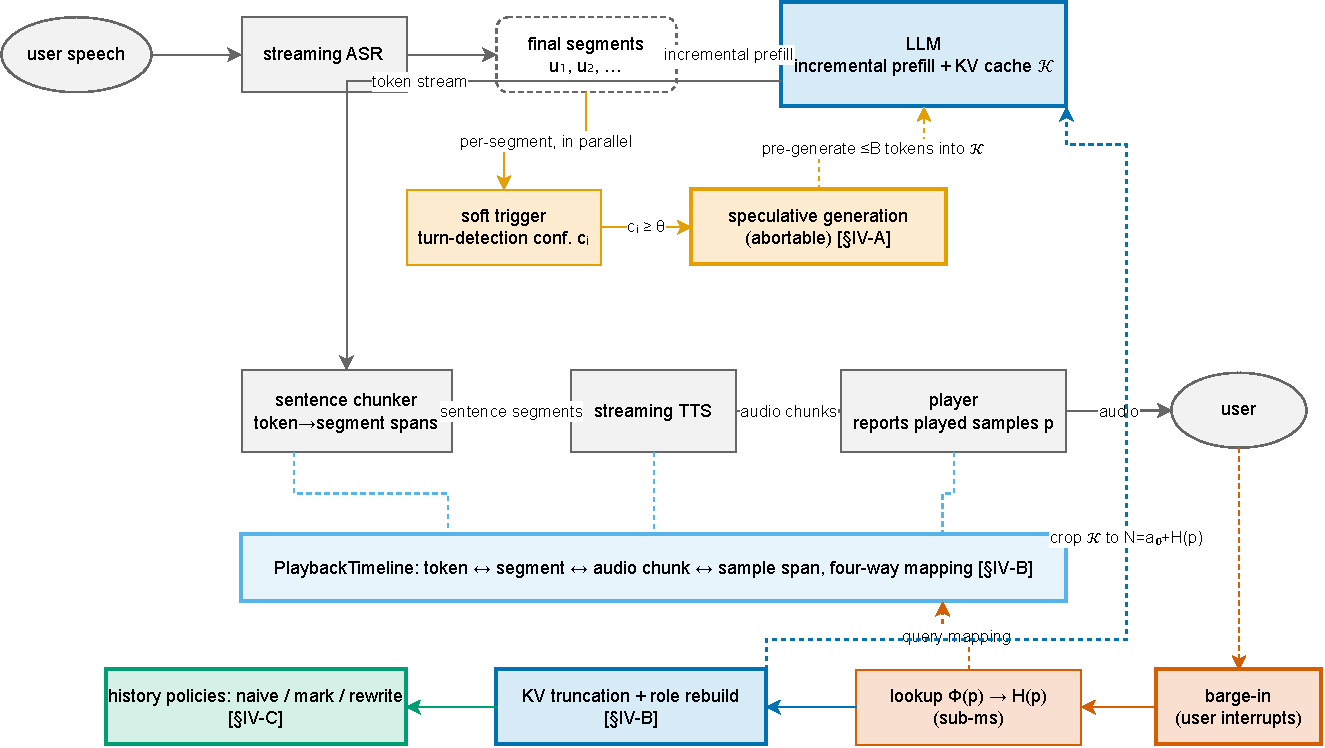
\includegraphics[width=0.9\textwidth]{fig4_1_en.pdf}
\caption{System architecture. Top: input pipeline and soft-trigger-driven speculative generation (Sec.~\ref{sec:spec}). Middle: output pipeline and the four-way mapping timeline (Sec.~\ref{sec:timeline}). Bottom: barge-in chain---lookup $\Phi(p)\!\rightarrow\!H(p)$, KV truncation + role rebuild (Sec.~\ref{sec:kv}), history policies (Sec.~\ref{sec:hist}).}
\label{fig:arch}
\end{figure*}

设计遵循两条原则：\textbf{(P1) 对话历史 = 用户实际听到的内容}（该原则本身已见于商用系统，见第二章；本文给出其在开源级联栈上的显式 KV 机制实现）；\textbf{(P2) 以冗余计算换交互流畅度}，且冗余可测、可调（\S\ref{sec:form} 浪费率与权衡曲线）。

\subsection{推测生成调度（贡献 1）}\label{sec:spec}

\subsubsection{软触发的两阈值机制}
传统端点检测输出二值决策，误判即造成"抢答"或"迟钝"。本文以现成的 turn 检测模型（TEN Turn Detection~\cite{ten_turn}）输出连续置信度 $c_i = \mathrm{conf}(u_1 \dots u_i) \in [0,1]$，配两个阈值：
\begin{itemize}
  \item \textbf{推测阈值 $\theta$}（激进）：$c_i \ge \theta$ 即启动\textbf{推测生成}——注入 assistant 角色标记并预生成至多 $B$ 个 token（$B$ 为推测预算，限制单次作废成本；不用 $\kappa$ 以免与 Cohen's $\kappa$ 混淆）；
  \item \textbf{提交语义}：确定性协议下以用户真实说完为提交事件；实际部署中可另设保守阈值控制 TTS 播出时机（播出前的推测对用户不可见，作废零感知）。
\end{itemize}
软触发为文本侧模型，其推理与该片段的 KV prefill \textbf{并行执行}（prefill 是既有开销），故触发判断不增加端到端延迟。

\subsubsection{推测-作废状态机}
对每个到达的用户片段 $u_i$：(1) \textbf{作废}（若存在活跃推测）：新片段到达意味着用户仍在说话、早前触发是误判 $\rightarrow$ 将 KV 截断回推测起点 $b$（user 内容末尾、assistant 标记之前），推测产出计入浪费；(2) \textbf{prefill} $u_i$（user 角色保持打开，增量累积）；(3) \textbf{评估} $c_i$；$c_i \ge \theta$ $\rightarrow$ 记录推测起点 $b := |\mathcal{K}|$，注入 assistant 标记，预生成 $\le B$ token 并缓存。

用户真实说完时：若有存活推测，缓存 token 立即可用（$\mathrm{TTFT}_{\text{eff}} \approx 0$），继续生成余量；否则现场触发生成（支付全额 TTFT）。存活的推测正是"最后一个片段触发、其后再无语音"的那次——其计算被端点静默窗掩盖。作废的正确性依赖 \S\ref{sec:crop} 的合法截断：推测回滚是"播放期打断"的退化情形（$p=0$，历史回滚到 $H=0$）。

推测-作废状态机如图~\ref{fig:fsm} 所示。该机制把端点判断从硬决策转化为可调旋钮：$\theta$ 扫描给出 $(\rho, \mathrm{TTFT}_{\text{eff}})$ 权衡前沿（\S\ref{sec:e2}），系统按算力预算选择工作点。

\begin{figure}[t]
\centering
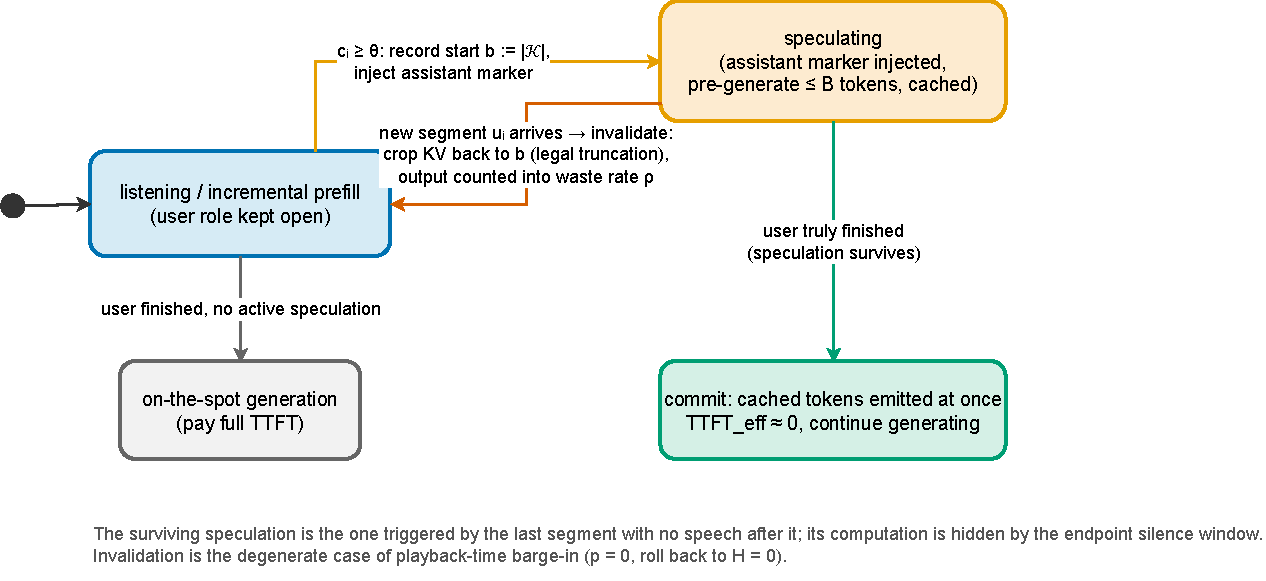
\includegraphics[width=\linewidth]{fig4_2_en.pdf}
\caption{The speculate-invalidate state machine. A newly arrived segment invalidates the active speculation and crops KV back to the speculation start $b$; if the user has truly finished and the speculation survives, cached tokens are emitted immediately with $\mathrm{TTFT}_{\mathrm{eff}}\approx0$.}
\label{fig:fsm}
\end{figure}

\subsection{播放感知的 KV 缓存管理（贡献 2，核心）}\label{sec:kv}

\subsubsection{四向映射时间轴}\label{sec:timeline}
反向映射 $\Phi$（定义~\ref{def:phi}）由\textbf{播放时间轴}（PlaybackTimeline）支撑：以片段记录为主轴的追加式结构，每条记录维护
$$\langle \text{片段 } f_j,\ \text{token 区间 } [\mathrm{ts}, \mathrm{te}),\ \text{音频块列表},\ \text{采样区间 } [\mathrm{ss}, \mathrm{se}),\ \text{状态} \rangle,$$
状态机为 推测 $\rightarrow$ 合成中 $\rightarrow$ 已入队 $\rightarrow$ 播放中 $\rightarrow$ 已播完 / 已作废。三个生产者分别写入自己的映射维度（生成线程写 token$\leftrightarrow$片段、TTS 线程写片段$\leftrightarrow$音频块并推进采样轴、播放线程原子更新已播采样数 $p$），打断到达时反查按采样区间定位片段（计数语义 $\mathrm{ss} < p \le \mathrm{se}$，边界处恰好判为"完整听完"）。片段数为轮级小量，全表单锁 + 播放游标无锁即满足亚毫秒反查（\S\ref{sec:a1}）。时间轴结构与反查过程如图~\ref{fig:timeline} 所示。

\begin{figure*}[t]
\centering
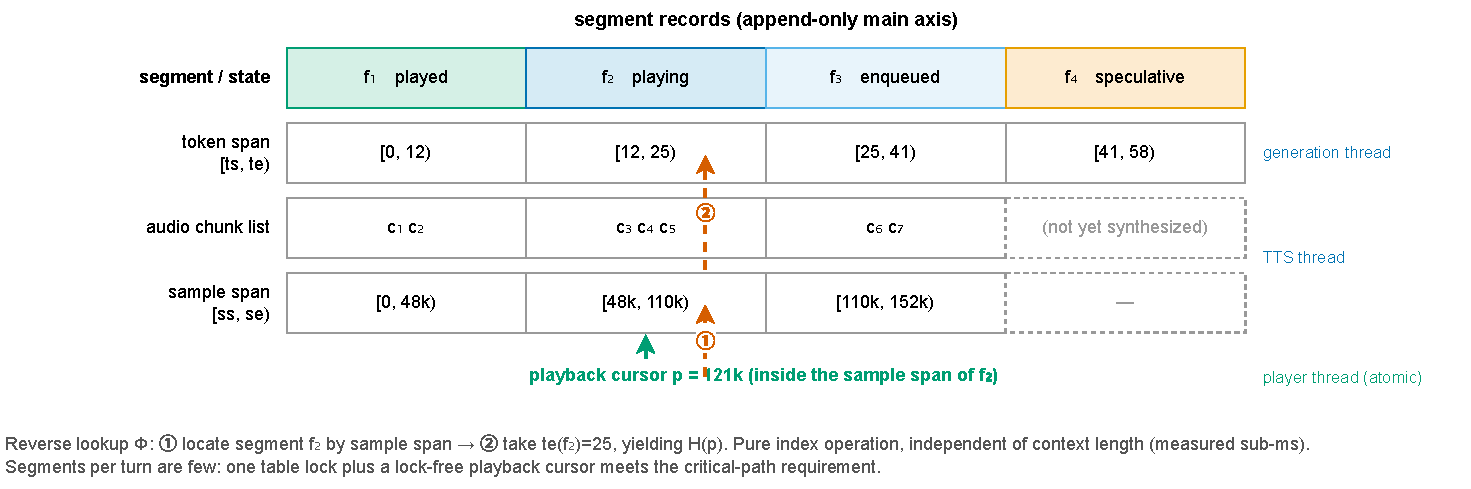
\includegraphics[width=0.82\textwidth]{fig4_3_en.pdf}
\caption{The four-way mapping timeline and reverse lookup $\Phi$. Segment records form the append-only main axis; three producer threads write the token-span, audio-chunk, and sample-span dimensions respectively. On barge-in, the segment is located by sample span and its $\mathrm{te}$ yields the heard boundary $H(p)$---a pure index operation.}
\label{fig:timeline}
\end{figure*}

\textbf{token 区间的来源}：断句器不感知 token。本文以\textbf{非空白字符计数对齐}建立句子片段与 token 区间的映射——向断句器供给 token 文本时累计非空白字符前缀和，片段产出时按其非空白字符数在前缀和上二分定位末 token。该映射对断句器的空白归一化免疫，且可验证无损（片段拼接与解码文本的非空白字符严格守恒）。

\subsubsection{合法的 KV 截断}\label{sec:crop}
打断时刻，$\Phi(p)$ 给出听到边界 $H(p)$，KV 截断至绝对位置 $N = a_0 + H(p)$。满足定义~\ref{def:legal} 的三个条件需要同步维护三份状态：(1) KV 张量截断（\texttt{DynamicCache} 的序列维切片~\cite{hf_kvcache}）；(2) \textbf{注意力掩码同步截短至 $N$}——掩码长度是后续 past length 的事实来源，仅截 KV 不截掩码会使位置编码整体错位（一期审查确认的首要陷阱）；(3) 序列长度与本轮 assistant token 账本同步更新，后续 prefill 的位置编码自 $N$ 起显式重算。截断本身是张量切片（亚毫秒），构成"打断即停"的全部关键路径开销。

\subsubsection{角色边界重建}\label{sec:role}
KV 是连续序列，角色信息仅存在于 chat template 的特殊标记中；截断落点在 assistant 内容中间，直接续写会破坏 prompt 结构。本文从 tokenizer 的 chat template 推导出\textbf{角色切换串}（如 ChatML 的 \texttt{<|im\_end|>\textbackslash n<|im\_start|>user\textbackslash n}），截断后将其作为普通文本增量 prefill 进 KV——复用与流式 prefill 完全相同的显式掩码/位置编码机制，无需特殊算子。角色重建（一次数 token 的小 prefill，数十毫秒）\textbf{不在打断响应关键路径上}：打断只需"停播 + 截断"，重建可延迟到下一轮用户输入到达前执行。截断与角色重建的完整过程如图~\ref{fig:crop} 所示。

\begin{figure*}[t]
\centering
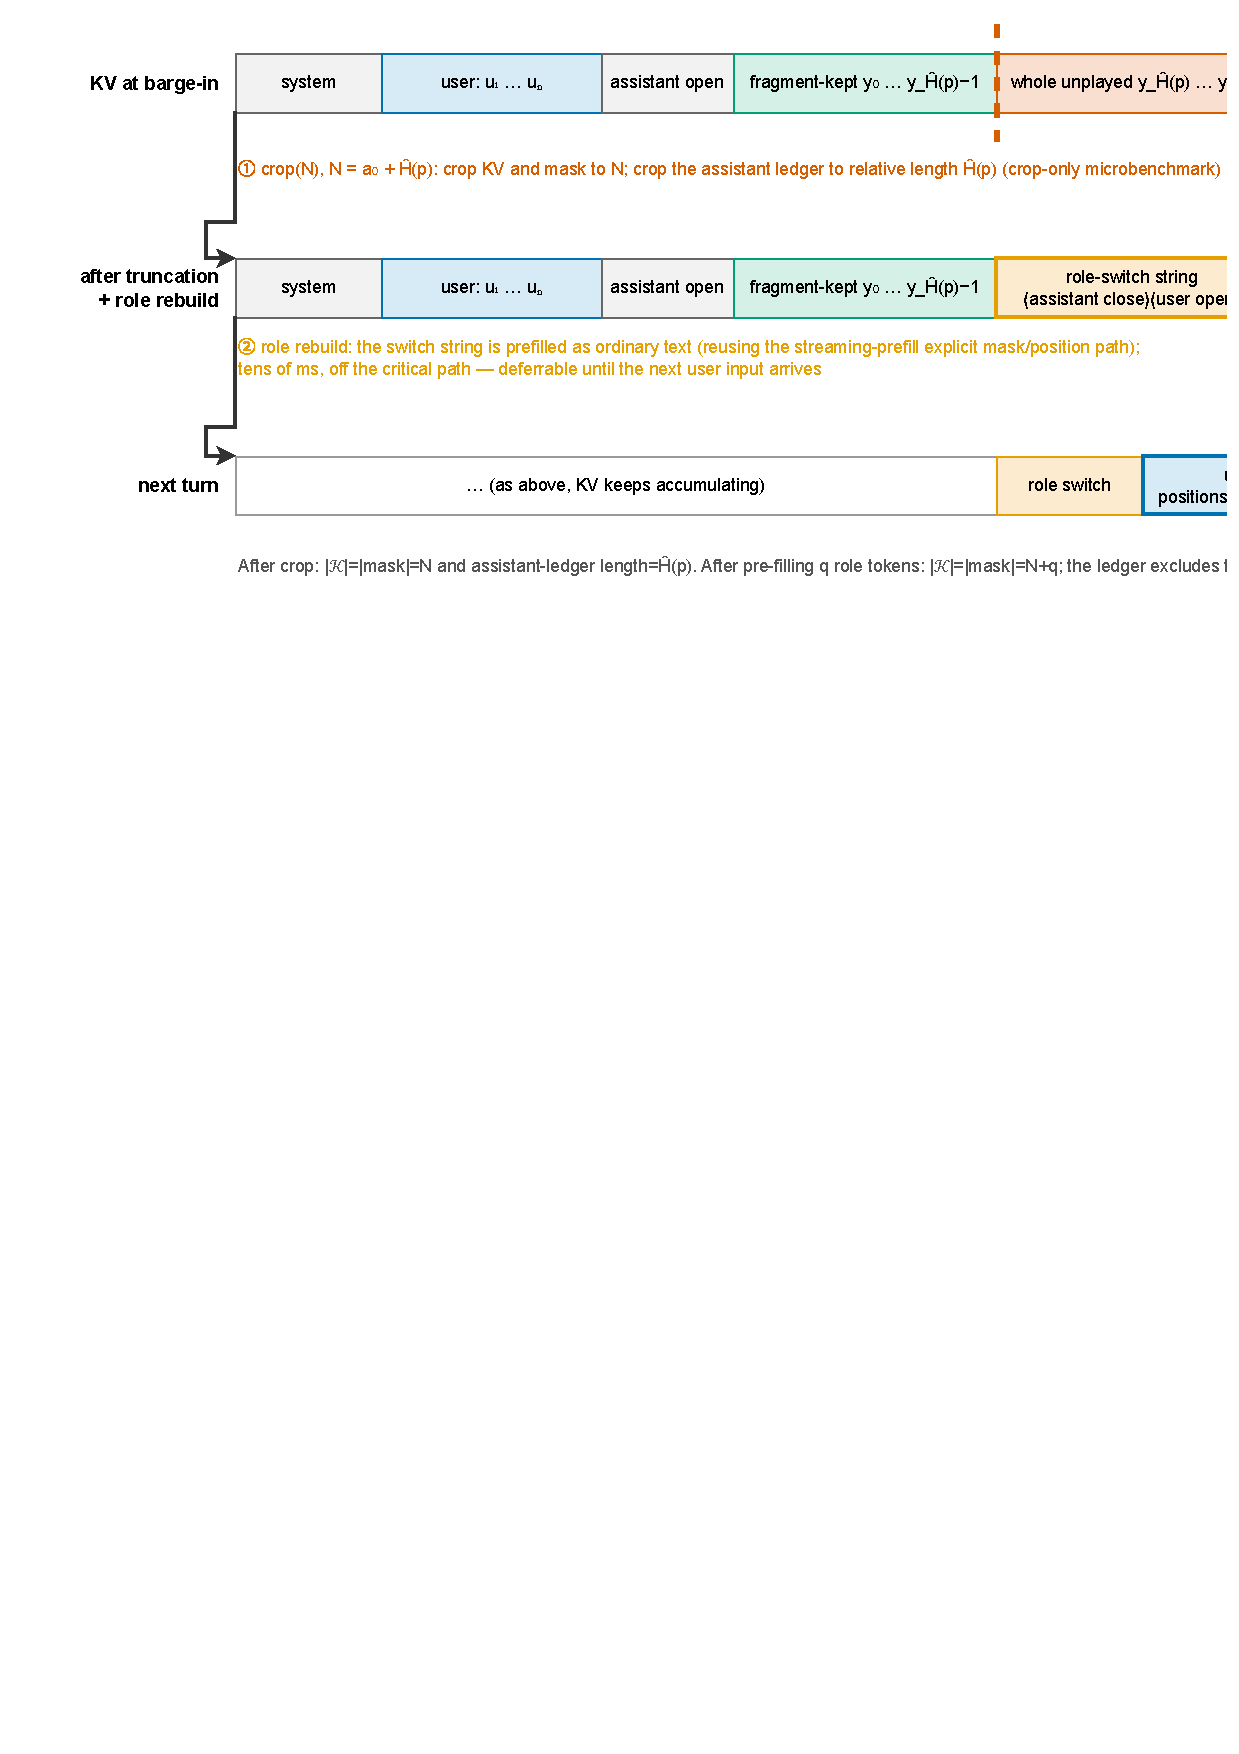
\includegraphics[width=0.82\textwidth]{fig4_4_en.pdf}
\caption{KV truncation and role-boundary rebuild. \textcircled{1} At barge-in the cache is cropped along the heard boundary to $N=a_0+H(p)$; unheard content leaves both KV and history---the critical path is this single sub-ms step. \textcircled{2} The role-switch string is prefilled as ordinary text, off the critical path. \textcircled{3} The next user turn continues with position encodings contiguous from $N$.}
\label{fig:crop}
\end{figure*}

由此，多轮对话在单一 KV 上持续累积：user 增量 prefill $\rightarrow$ assistant 边生成边累积（生成循环将每个新 token 的 KV、掩码与 token id 写回同一缓存对象，使 assistant 侧 KV 成为可截断的一等状态——这是对一期"生成不回写"设计的关键扩展）$\rightarrow$ 打断或说完 $\rightarrow$ 截断/收尾 $\rightarrow$ 角色重建 $\rightarrow$ 下一轮。

\subsubsection{与三条基线的对比语义}
\textbf{generation 截断}（B-gen）：保留全部已生成内容，历史含 $y_{H(p)+1..G}$ 的未听部分——\S\ref{sec:e3} 证明其半数场景引发未听内容复现；\textbf{重新 prefill}（B-noKV）：放弃 KV、以文本重建历史——成本随上下文线性增长（\S\ref{sec:a1}，8k 时 1.86\,s vs 亚毫秒）；\textbf{synthesis 截断}：以合成指针 $s$ 为界，在同步合成下与 generation 等价，异步流式合成下介于两者之间（本文不主张已验证）。

\subsection{被打断历史的处理策略（贡献 3，探索性）}\label{sec:hist}
播放感知截断使历史精确等于所听内容，但半截片段场景下历史以语义不完整的半句结尾。本文比较三种策略（均在 playback 截断之上）：
\begin{itemize}
  \item \textbf{朴素截断}：不作处理；
  \item \textbf{标记法}：在被截断内容尾部追加打断标记（如省略号），零延迟零模型成本，向模型显式提示"此处被打断"；
  \item \textbf{重写法}：仅当截断落于语义不完整处（partial）时，调用轻量模型（Qwen3-0.6B~\cite{qwen3}）将半句改写为自然收尾版本，\textbf{约束不得新增信息}（否则历史将包含"没说过的话"，比 B-gen 更糟）；KV 层面以重写文本替换被打断的 assistant 段（截断回 $a_0$ + prefill 重写文本），复用率相应下降但重算段很短。重写与用户打断后的说话期并行，P90 延迟 $<1$\,s 可被完全隐藏（\S\ref{sec:a2}）。
\end{itemize}
实验结果（\S\ref{sec:a2}）如实报告：在 7B 主模型下三策略连贯性无显著差异，重写未表现出收益；本文将其定位为机制可行性的探索性验证。

% ==================================================== 第五章
\section{系统实现}\label{sec:impl}
本章体现工程贡献与可复现性：模块结构、关键实现点、部署与验证方法学。全部代码开源于项目仓库。

\subsection{总体结构与代码地图}
系统在一期代码基（流式 ASR 基于 Whisper~\cite{whisper}、LLM 增量预填充）上新增四个模块组，总计约 2500 行，模块结构如表~\ref{tab:modules} 所示。

\begin{table}[t]
\caption{Module map of the open-source implementation}
\label{tab:modules}
\centering
\scriptsize
\begin{tabular}{@{}p{0.36\linewidth}p{0.42\linewidth}p{0.12\linewidth}@{}}
\toprule
Module & Responsibility & Sec. \\
\midrule
\texttt{dialogue/timeline.py} & four-way mapping timeline, reverse lookup $\Phi$ & \S\ref{sec:timeline} \\
\texttt{llm/stream\_llm\_} \texttt{inference.py} (ext.) & truncatable KV (AccumKVCache), legal crop, role rebuild & \S\ref{sec:crop}--\ref{sec:role} \\
\texttt{tts/} & chunker + token-span alignment; StreamingTTS; CosyVoice2 adapter & \S\ref{sec:timeline} \\
\texttt{dialogue/trigger.py}, \texttt{rewriter.py} & soft trigger; history rewriting & \S\ref{sec:spec}, \ref{sec:hist} \\
\texttt{dialogue/} \texttt{orchestrator.py} & orchestration loop, barge-in chain, metric instrumentation & all \\
\texttt{experiments/scripts/} & 6 experiment harnesses, calibration, LLM judge, TTS profiling & \S\ref{sec:eval} \\
\bottomrule
\end{tabular}
\end{table}

\subsection{关键实现点}
\textbf{可截断的 assistant 侧 KV}　一期的生成循环不将新 token 的 KV 回写调用方，无法支持截断与多轮。本文扩展为：生成循环每步将 KV、注意力掩码、token id 同步写回统一容器（AccumKVCache，显式断言 \texttt{DynamicCache} 类型），并记录本轮 assistant 起点 $a_0$ 与 token 账本——账本即时间轴 token 维的数据源。截断实现为 \texttt{DynamicCache.crop(N)} + 掩码切片 + 账本裁剪三者的原子组合；三份长度的一致性（定义~\ref{def:legal} 条件 1）以运行时不变式检查覆盖全部实验路径。

\textbf{角色切换串的推导}　不硬编码模板标记：初始化时以哑消息套用 chat template，差分提取"生成提示符"（user$\rightarrow$assistant）并变换得到 assistant$\rightarrow$user 切换串，兼容 ChatML 系模板；注入走与流式 prefill 相同的显式掩码/位置编码路径（\S\ref{sec:role}）。

\textbf{断句对齐的鲁棒性}　非空白字符前缀和对齐（\S\ref{sec:timeline}）之外的两个边界处理：纯空白句直接跳过（否则兜底推进会挪用下一片段首 token、使截断点偏移）；区间末端钳制到实际生成数（防越界截断）。半截片段的严格口径切分（strict）按播放采样比例切文本并吸附词边界，避免半词污染引用检测。

\textbf{确定性实验协议}　打断由 harness 程序注入（受控播放比例/片段边界），播放器为确定性时钟：TTS 时序画像（每字符采样数、首块延迟、RTF）取真机 benchmark 值驱动模拟——所有一致性/效率结论与真机时序等价且完全可复现；mouth-to-ear 为画像建模值并如实标注（\S\ref{sec:e1}）。

\textbf{指标埋点}　每轮落盘：8 个关键时间戳（说完/触发/首 token/首块/首播/打断注入/停播/截断完成）、双口径 TTFT、推测计数与浪费、KV 复用计数、时间轴快照（token$\leftrightarrow$片段$\leftrightarrow$音频块$\leftrightarrow$采样区间全表）——第三章每个指标都能从落盘数据复算。

\subsection{部署}
部署配置如表~\ref{tab:deploy} 所示。三个 LLM 实例独立部署、不复用权重，模拟真实多服务工程。全部模型配置经环境变量集中管理，验证环境（0.5B 开发替身）与实验环境切换零改码。

\begin{table}[t]
\caption{Deployment configuration}
\label{tab:deploy}
\centering
\resizebox{\linewidth}{!}{%
\begin{tabular}{@{}llll@{}}
\toprule
Role & Model & Size & Placement \\
\midrule
Main LLM & Qwen2-7B-Instruct~\cite{qwen2} & 7B & GPU 0 ($\sim$14\,GB+KV) \\
Soft trigger & TEN Turn Detection~\cite{ten_turn} & 7.6B & GPU 1 ($\sim$15\,GB) \\
History rewriter & Qwen3-0.6B~\cite{qwen3} & 0.6B & GPU 1 \\
LLM judge (eval only) & Mistral-7B-v0.3~\cite{mistral7b} & 7B & GPU 1 (shared) \\
Streaming TTS & CosyVoice2~\cite{cosyvoice2} & 0.5B & GPU 1 (own env) \\
\bottomrule
\end{tabular}}
\end{table}

\subsection{验证方法学}
代码可信度依三道防线建立：(i) \textbf{组件级 smoke 测试}九套（时间轴边界语义、KV 三长度不变式、断句守恒、推测状态机、端到端打断链路等），全部随实验环境回归；(ii) \textbf{两轮对抗式代码审查}——第一轮发现三个将污染实验数字的缺陷（E3 指标口径、E1 对照公平性、断句越界）并修复，第二轮验证修复并清理五个次要项，全程记录于决策日志；(iii) \textbf{数据级验证}——干净边界注入组 103/103 样本 strict 残余为零（\S\ref{sec:e3}），从实验数据侧印证截断语义实现正确。

% ==================================================== 第六章
\section{实验与结果分析}\label{sec:eval}

\subsection{实验设置}
\textbf{硬件与部署}　实验机为 2$\times$ NVIDIA RTX 3090（24\,GB）：卡 0 部署主 LLM；卡 1 部署软触发、重写与裁判模型。全部延迟数字在该配置下测得。

\textbf{模型}　主 LLM 为 Qwen2-7B-Instruct~\cite{qwen2}（与一期实验对齐）；软触发为 TEN Turn Detection~\cite{ten_turn}（7.6B，文本侧，输出 finished/unfinished/wait 类别词概率作为连续置信度，实测标定成对正确率 AUC$=1.00$）；历史重写模型为 Qwen3-0.6B~\cite{qwen3}；LLM 裁判为 Mistral-7B-Instruct-v0.3~\cite{mistral7b}（\textbf{与主 LLM 不同家族}，避免同族偏袒）；流式 TTS 为 CosyVoice2-0.5B~\cite{cosyvoice2}。TTS 时序画像取真机实测：3175 采样/非空白字符（24\,kHz，约 7.5 字符/秒语速）、首块合成延迟 2433.6\,ms、合成实时率 RTF$=$0.513。需要说明，首块延迟为 3090 无 TensorRT 加速的实测值，官方报告 A100+TensorRT+fp16 下可至约 45\,ms，\S\ref{sec:e1} 据此做部署条件敏感性讨论。

\textbf{数据}　自 MultiWOZ 2.1~\cite{multiwoz21} 派生（固定随机种子）：103 条多轮对话（每条 $\ge$3 个 user 轮，用于 E3/A2）与 100 条子句切分话语（切分严格无损，段边界即停顿点，用于 E1/E2）。语种为英文。

\textbf{打断注入协议}　确定性程序注入（\S\ref{sec:form}）：对每条被打断轮，分别在播放比例 25\%、50\%、75\%（多落于片段中间，构成半截片段）与片段干净边界（对照）注入打断，"用户听到的内容"以注入时刻播放指针为真值，全部实验可复现。

\textbf{被测条件}　System A（非流式基线：说完$\rightarrow$全量 prefill$\rightarrow$生成完$\rightarrow$整段合成）；B-ours（本文方法：playback 截断）；B-gen（对照：generation 截断，历史保留全部已生成内容）。合成位置截断（B-syn）在同步合成模拟下与 B-gen 等价，本文不将其作为已验证条件。

\subsection{E3：多轮一致性（主结果）}\label{sec:e3}
每条件 $n{=}412$（103 对话 $\times$ 4 注入位置）。表~\ref{tab:consistency} 给出未听内容引用率的双口径、双检测器结果。

\begin{table}[t]
\caption{Unheard-content reference rate (E3 main result). B-ours loose 0\% is a constructive guarantee; Cohen's $h$: 1.59 = very large, 0.47 = medium.}
\label{tab:consistency}
\centering
\scriptsize
\setlength{\tabcolsep}{3.5pt}
\begin{tabular}{@{}lllll@{}}
\toprule
Criterion / detector & B-ours & B-gen & Fisher exact & $h$ \\
\midrule
loose / rule & \textbf{0.0\% (0/412)} & \textbf{51.0\% (210/412)} & $1.8{\times}10^{-79}$ & 1.59 \\
strict / rule & 51.0\% (210/412) & 73.3\% (302/412) & $5.0{\times}10^{-11}$ & 0.47 \\
loose / judge & \textbf{0.0\% (0/412)} & 2.7\% (11/412) & $9.1{\times}10^{-4}$ & --- \\
strict / judge & 2.4\% (10/412) & 2.9\% (12/412) & 0.83 (n.s.) & --- \\
\bottomrule
\end{tabular}
\end{table}

\textbf{主结论}（写作红线：loose 口径下 B-ours 的 0\% 是\textbf{机制的构造性保证而非实验发现}——历史中不存在未听片段，引用无从发生；实验量化的是对照方法的失败率）：
\begin{enumerate}
  \item \textbf{朴素的 generation 截断在半数场景下引发未听内容复现}：规则口径 51.0\% 的后续回复复用了用户从未听到的词面内容；即使按最保守的裁判口径（仅特定信息引用），仍有 2.7\% 的轮次让模型"引用了自己从未说出口的话"，两把尺子下差异均显著（$p<10^{-3}$）。
  \item \textbf{打断越早，危害越大}：B-gen 的 loose 引用率随注入位置单调递减——25\% 处 85.4\%（88/103）、50\% 处 48.5\%、75\% 处 20.4\%；干净边界处 49.5\%。未听内容越多，被复现的概率越高，与直觉一致，如图~\ref{fig:positions} 所示。
  \item \textbf{片段粒度量化误差的后果可忽略}：strict 口径下 B-ours 存在半截片段尾部残余（定义~\ref{def:eps}），规则检测器报 51.0\%——但这是词面重叠上界；裁判口径下 B-ours strict 仅 2.4\%，且与 B-gen（2.9\%）无显著差异（$p=0.83$）。即：以片段为截断原子的工程取舍，在"特定信息被错误引用"的意义上没有可测量的额外代价。
  \item \textbf{截断语义精确成立}：干净边界注入组 103/103 样本的 strict 残余为零，与定义~\ref{def:boundary} 的边界语义一致，可视为机制实现正确性的数据级验证。
\end{enumerate}

\begin{figure}[t]
\centering
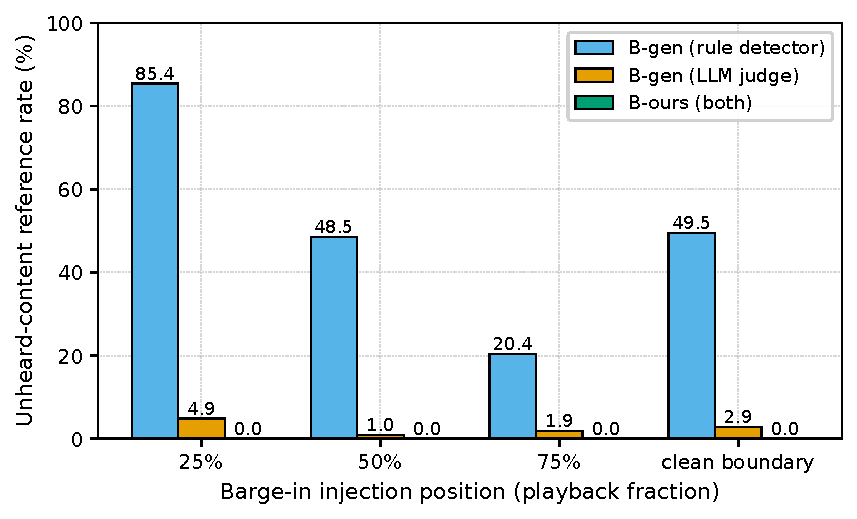
\includegraphics[width=\linewidth]{fig6_1_en.pdf}
\caption{Unheard-content reference rate by injection position. B-gen decreases monotonically with later interruption; B-ours is zero under both criteria---a constructive guarantee of the mechanism, not a statistical finding.}
\label{fig:positions}
\end{figure}

\textbf{检测器方法学}　规则检测器与 LLM 裁判在真实数据上一致性很低（Cohen's $\kappa\approx0.05$；开发用小样本上为 0.71）。原因是 MultiWOZ 任务域高频词（hotel、book、train 等）使词面线索在域内自然复现，规则检测器系统性过触发。因此本文将规则口径解释为\textbf{表面重叠上界}、裁判口径为\textbf{特定引用下界}，真值介于其间；关键在于\textbf{两把尺子下 B-ours 均不劣于 B-gen，且 loose 口径双双为零}，主结论对检测器选择鲁棒。

为仲裁两把尺子，按判定组合分层抽取 37 条样本进行人工标注（判定标准与裁判一致：仅特定事实/数字/措辞的引用计为"是"）。结果（表~\ref{tab:arbitration}）：人工与\textbf{裁判}在 loose 口径中等偏强一致（一致率 84.6\%，$\kappa=0.649$），而与\textbf{规则检测器}的一致性不优于随机（一致率 30.8\%，$\kappa=-0.073$）——支持以裁判口径为正文主数字、规则口径仅作上界呈现。尤为重要的是，\textbf{strict 口径的 24 条样本中人工判定无一构成特定引用（0/24）}：片段级截断粒度引入的量化误差尾部（定义~\ref{def:eps}）在人类判定下不产生可感知的一致性损害，为第四章"以片段为截断单位"的设计取舍提供了实证辩护。

\begin{table}[t]
\caption{Human arbitration ($n{=}37$, stratified over judgment combinations)}
\label{tab:arbitration}
\centering
\begin{tabular}{llcc}
\toprule
Comparison & Criterion & Agreement & Cohen's $\kappa$ \\
\midrule
Human vs.\ LLM judge & loose ($n{=}13$) & 84.6\% & \textbf{0.649} \\
Human vs.\ rule detector & loose ($n{=}13$) & 30.8\% & $-0.073$ \\
Human "specific reference" & strict ($n{=}24$) & --- & 0/24 \\
\bottomrule
\end{tabular}
\end{table}

\subsection{E2：推测浪费率–TTFT 权衡曲线（核心图）}\label{sec:e2}
TEN 软触发阈值按实测置信度分布标定后扫描九点（含"永不推测"哨兵）。结果见表~\ref{tab:sweep} 与图~\ref{fig:frontier}。

\begin{table*}[t]
\caption{Soft-trigger threshold sweep ($n{=}100$ per point)}
\label{tab:sweep}
\centering
\begin{tabular}{lccccccccc}
\toprule
Threshold $\theta$ & 0.005 & 0.198 & 0.391 & 0.583 & 0.776 & 0.85 & 0.92 & 0.969 & 1.1 (never) \\
\midrule
Waste rate $\rho$ & 29.2\% & 16.2\% & 14.4\% & 13.6\% & 11.5\% & 10.7\% & 4.5\% & 0.8\% & 0\% \\
$\mathrm{TTFT}_{\text{eff}}$ (ms) & 0.5 & 0.1 & 0.6 & 1.1 & 3.9 & 5.8 & 12.1 & 29.3 & 48.5 \\
Survival rate & 100\% & 100\% & 99\% & 98\% & 92\% & 88\% & 75\% & 39\% & 0\% \\
\bottomrule
\end{tabular}
\end{table*}

\begin{figure}[t]
\centering
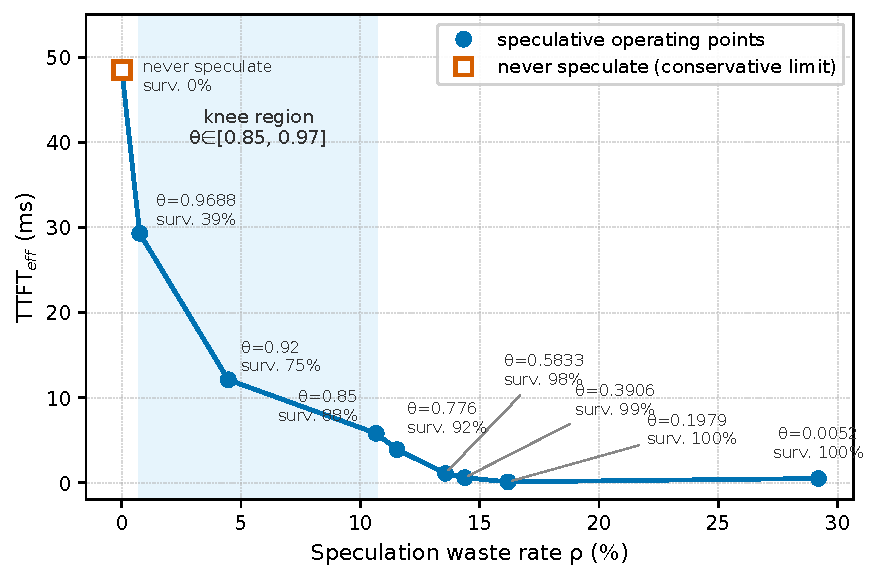
\includegraphics[width=\linewidth]{fig6_2_en.pdf}
\caption{Speculation waste rate vs.\ $\mathrm{TTFT}_{\mathrm{eff}}$: a continuously tunable frontier; the open square is the never-speculate conservative limit.}
\label{fig:frontier}
\end{figure}

\textbf{分析}　曲线呈单调权衡且存在明显拐点区（$\theta\in[0.85, 0.97]$）：$\theta=0.92$ 时以 4.5\% 的冗余计算换取 $\mathrm{TTFT}_{\text{eff}}$ 从 48.5\,ms 降至 12.1\,ms（$-75\%$）；$\theta=0.969$ 时浪费率仅 0.8\% 仍获 40\% 的延迟收益。这验证了 \S\ref{sec:form} 的设计命题——\textbf{端点判断从硬决策变为可调的连续旋钮}，系统可按算力预算选择工作点。激进端（$\theta\le0.4$）浪费率 14--29\% 而 $\mathrm{TTFT}_{\text{eff}}\approx0$：推测几乎总在用户说完前就绪。注意 7B 模型下"不推测"的 TTFT 全额仅 48.5\,ms（得益于一期流式 prefill 已消除上下文编码开销），故本实验的收益比例（$-75\%$ $\sim$ $-99\%$）比绝对毫秒数更具外推意义；对更大模型或更长回复前缀，绝对收益将同步放大。本表 records 级数据同时构成消融 A3（激进度扫描）。

\subsection{E1：端到端延迟}\label{sec:e1}
$n{=}100$，B-ours 取 $\theta=0.391$ 工作点。TTFT 口径（真实测量）：System A 平均 27.4\,ms，B-ours $\mathrm{TTFT}_{\text{eff}}$ 平均 \textbf{0.6\,ms}（改善 97.9\%）——推测存活使 token 在用户说完时几乎总已就绪。

mouth-to-ear 口径（\textbf{建模值}：首片段就绪时刻 + TTS 首块延迟，画像为 3090 实测）：A 为 9080\,ms（须等全部生成 + 整段合成），B-ours 为 2482\,ms，其中 2434\,ms 由 TTS 首块合成延迟主导。\textbf{部署条件敏感性}：该首块延迟强依赖推理加速条件——按官方 A100+TensorRT 报告值（$\approx$45\,ms）外推，B-ours 的 mouth-to-ear 可至约 100\,ms 量级，而 System A 的"等全部生成+整段合成"是结构性成本、随回复长度线性增长，不随 TTS 加速消失。如图~\ref{fig:e2e} 所示，建模量与实测量分别标注。

\begin{figure}[t]
\centering
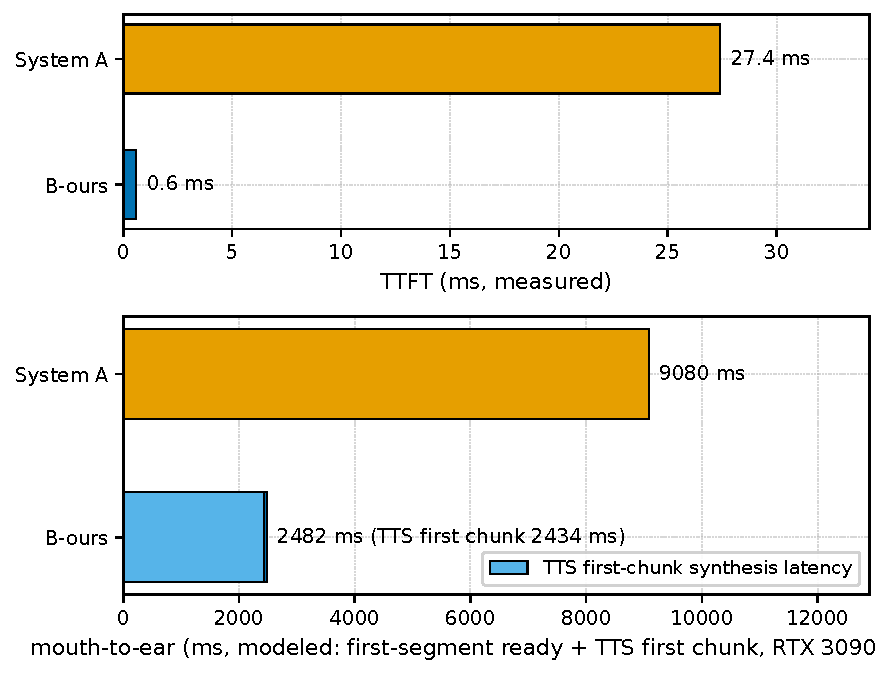
\includegraphics[width=\linewidth]{fig6_3_en.pdf}
\caption{End-to-end latency. Top: TTFT (measured). Bottom: mouth-to-ear (modeled: first-segment ready + TTS first chunk, RTX 3090 profile); of B-ours' 2482\,ms, 2434\,ms is TTS first-chunk synthesis latency.}
\label{fig:e2e}
\end{figure}

\subsection{A1：KV 复用收益与打断响应延迟（7B）}\label{sec:a1}
截断路径与重新 prefill 的对比如表~\ref{tab:kvreuse} 与图~\ref{fig:kvreuse} 所示。

\begin{table}[t]
\caption{Truncation path vs.\ re-prefill (median, ms)}
\label{tab:kvreuse}
\centering
\resizebox{\linewidth}{!}{%
\begin{tabular}{lccccc}
\toprule
Context length (tokens) & 275 & 1k & 2k & 4k & 8k \\
\midrule
Lookup + crop (critical path) & \multicolumn{5}{c}{0.31--0.34 (near-constant)} \\
Role rebuild (off critical path) & \multicolumn{5}{c}{25--47} \\
Re-prefill & 72 & 235 & 459 & 891 & 1863 \\
Speedup & 2.8$\times$ & 8.6$\times$ & 15.3$\times$ & 25.2$\times$ & \textbf{39.7$\times$} \\
\bottomrule
\end{tabular}}
\end{table}

\begin{figure}[t]
\centering

\includegraphics[width=\linewidth]{fig6_4_en.pdf}
\caption{Barge-in response paths vs.\ re-prefill across context lengths (log--log). Lookup+crop is sub-ms and length-independent; role rebuild is off the critical path; re-prefill grows nearly linearly (39.7$\times$ at 8k).}
\label{fig:kvreuse}
\end{figure}

\textbf{barge-in 响应延迟恒为亚毫秒级且与上下文长度无关}——反查（定义~\ref{def:phi} 的 $\Phi$）为纯索引操作、截断为张量切片；角色重建可延迟到下一轮输入前执行，不在"打断即停"的关键路径上。作为对照，放弃 KV 复用而对听到边界前的完整上下文重新 prefill 的成本随长度线性增长，8k 上下文时达 1.86\,s——多轮语音对话的上下文天然持续增长，KV 复用收益随对话进行单调扩大。

\subsection{A2：被打断历史的三种处理策略}\label{sec:a2}
$n{=}100$/策略，裁判连贯性评分（1--5）：朴素截断 3.76、重写法 3.62、标记法 3.29；重写延迟 mean 639\,ms / P90 937\,ms / max 1165\,ms。

\textbf{诚实报告}：重写法未优于朴素截断（Wilcoxon 配对检验 $p=0.32$，无显著差异），标记法反而更低。可能原因：(i) 7B 主模型对半句历史已有较强鲁棒性，重写收益空间小；(ii) 0.6B 重写模型的改写质量有限；(iii) 单裁判单点评分的敏感度不足。工程侧结论仍成立——重写延迟 P90$<$1\,s，可隐藏于用户打断后的说话期内（架构上并行执行），且 KV 复用率按重算段比例可控。据此，本文将历史自然化重写定位为\textbf{探索性结果}：机制可行、延迟可隐藏，但在本实验设置下未观察到一致性收益，留待更强重写模型与更细评价方式（如成对偏好）检验。

\subsection{结果小结}
\begin{itemize}
  \item \textbf{一致性（主张核心）}：playback 截断使历史与用户所听严格一致（loose 恒 0，构造性），对照方法在 51\%（词面）/2.7\%（特定引用）的场景引入未听内容复现；片段粒度量化误差在特定引用意义上无可测量代价（$p=0.83$）。
  \item \textbf{延迟}：推测生成把 $\mathrm{TTFT}_{\text{eff}}$ 压至亚毫秒–数毫秒并可按 $(\rho, \mathrm{TTFT})$ 曲线调节（拐点 $\theta\approx0.92$：4.5\% 浪费换 75\% 延迟削减）；打断响应亚毫秒且与上下文无关；KV 复用相对重 prefill 最高 39.7$\times$。
  \item \textbf{方法学}：双检测器夹逼 + 干净边界 103/103 零残余的实现验证，构成结果可信度的两道防线；重写策略如实报告为无显著收益的探索性结果。
\end{itemize}

% ==================================================== 第七章
\section{讨论}\label{sec:discussion}

\subsection{与商用系统的关系}
本文与 OpenAI Realtime、Azure Voice Live、LiveKit 的关系是\textbf{开源参考实现与闭源产品的互补}，而非能力有无之别（第二章表~\ref{tab:diff}）。差异集中在三处：其一，操作层次——商用系统删除受管理的转写条目，本文在 LLM 推理内部对 KV 缓存做显式截断，保留了跨轮 KV 复用带来的延迟收益（A1：8k 上下文处 39.7$\times$）；其二，位置来源——Azure 以"实时速度假设"估算、OpenAI 依赖客户端上报，本文由播放器回报采样计数并经反向映射精确到片段边界；其三，可检视性——本文的映射表、时间戳与截断决策全部落盘，实验可复现。需要强调的是，这些差异不支持"商用系统未实现该功能"的论断——它们实现了，且其转写级方案在其产品约束下是合理的工程选择。

\subsection{局限与效度威胁}
\textbf{一致性度量的仪器差异。}规则检测器在任务域（MultiWOZ 高频词）上系统性过触发，与人工仲裁一致性不优于随机（$\kappa=-0.073$）；LLM 裁判获得中等偏强的人工一致（$\kappa=0.649$）但样本量有限（37 条）。本文以"上界—下界—仲裁"三层协议缓解，但更大规模的人工标注将进一步收紧区间。

\textbf{重写策略未显收益。}A2 中 0.6B 重写模型的裁判连贯性（3.62）未超过朴素截断（3.76）。可能原因：7B 主模型对半句历史本就鲁棒；0.6B 重写引入的措辞变化反而稀释了上下文线索。这提示贡献 3 的价值依赖于主模型与重写模型的能力配比，作为扩展贡献如实报告。

\textbf{时序建模的等价性假设。}开发与部分实验以实测时长画像驱动的 Mock TTS 进行，其与真机的等价性仅限时序维度；mouth-to-ear 的正式数值来自真机画像（3090 无 TRT 首块 2434\,ms），与官方 A100+TRT 指标（45\,ms）相差两个数量级——硬件与推理栈对该指标影响极大，跨系统比较需谨慎。

\textbf{数据与语种范围。}实验限于英文任务型对话（MultiWOZ 派生）与程序注入的确定性打断；开放域对话、真实用户打断行为与中文场景（stanza 断句路径、CosyVoice2 中文合成）留待扩展。打断时机的固定比例注入覆盖受控但非自然分布。

\textbf{软触发的域适配。}TEN 在本文句式上可分性极强（标定 AUC$=1.00$），E2 的浪费主要来自派生数据中"句法近似完整"的假停顿；口语更强的犹豫、修正现象下阈值前沿的形状可能不同。

\subsection{可推广性}
机制层面的三个组件均不绑定具体模型栈：反向映射表只要求下游产出"片段$\rightarrow$音频块"的归属关系，任何句子级输入的流式 TTS 均可接入（StreamingTTS 接口）；KV 截断与角色重建依赖 transformers 的 \texttt{DynamicCache} 与 ChatML 类模板，适用于该生态的任意因果 LM；软触发仅需一个输出连续置信度的文本判断器。三进度指针的不变式~\eqref{eq:invariant} 与听到边界语义（定义~\ref{def:boundary}）对任何"生成快于播放"的级联系统成立，包括未来接入更低延迟 TTS 或更大主模型的配置。

% ==================================================== 第八章
\section{总结与展望}\label{sec:conclusion}

\subsection{全文总结}
本文面向级联式流式语音对话系统的打断场景，研究"系统所记的对话历史"与"用户实际听到内容"的一致性问题。在形式化"生成—合成—播放"三进度指针与听到边界语义的基础上，本文实现并验证了三项机制：以连续置信度双阈值驱动的\textbf{推测生成调度}（C1）、基于反向映射与显式 KV 截断的\textbf{播放感知上下文管理}（C2）、以及被打断历史的\textbf{三种处理策略}（C3），并将其整合为首个开源、可复现的级联式参考实现。

实验（7B 主模型、MultiWOZ 派生数据、专用 turn-detection 模型）表明：打断响应关键路径恒为亚毫秒级且与上下文长度无关，KV 复用相对重新预填充在 8k 上下文处加速 39.7 倍（A1）；推测调度以约 4.5\% 的 token 浪费将说完后的首 token 延迟从 48.5\,ms 降至 12.1\,ms，权衡前沿连续可调（E2）；在一致性上，播放感知截断将片段口径的未听内容引用率由构造保证为零，LLM 裁判口径下对照组仍有 2.7\% 的特定引用与 51\% 的表面重叠上界，人工仲裁（$\kappa=0.649$）支持裁判口径的可信度，且片段级截断粒度的量化误差在人工判定下未产生任何可感知引用（E3）。

方法学上，本文提出的"上界检测器—下界裁判—人工仲裁"三层一致性判定协议，以及对规则检测器在任务域过触发现象的定量揭示，对同类语音对话评测具有独立参考价值。

\subsection{展望}
\begin{itemize}
  \item \textbf{更细截断粒度}：在片段级机制之上探索词级甚至 token 级听到边界（需 TTS 提供词级时间戳），并量化其相对片段粒度的边际收益——本文 strict 口径 0/24 的人工判定提示该收益可能有限；
  \item \textbf{位置估计方式对比}：量化"实测播放缓冲"与商用系统"实时速度假设"在拥塞、变速等非理想播放条件下的一致性差异；
  \item \textbf{真实音频闭环与中文场景}：接入真实用户语音与流式 ASR 的全链路、扩展 CrossWOZ/中文合成路径；
  \item \textbf{端到端与级联的融合}：在保留级联可控性的前提下，借鉴帧同步思想进一步压缩三指针间隙。
\end{itemize}

一期工作打破了"延迟随语音长度线性增长"的约束，本文进一步回答了"被打断之后如何保持对话一致"的问题。两者共同表明：在可预见的将来，级联架构仍可通过细粒度的流式状态管理，不断逼近端到端系统的交互自然度，同时保有其模块化与推理能力优势。

\section*{致谢}
% TODO: 投稿前补充基金/致谢信息。
本文写作过程中使用大语言模型辅助文献检索核验、绘图脚本与语言润色；全部技术内容、实验与结论由作者完成并核验。

\bibliographystyle{IEEEtran}
\bibliography{references}

\end{document}
